\chapter{Evaluation}
\label{evaluation}
Im folgenden Kapitel werden Kernkonzepte von \texttt{SimpliFX} durch Quelltextbeispiele und eine Beispielanwendung erklärt. Außerdem wird eine Applikation erstellt, welche äquivalente Funktionalitäten wie die Beispielanwendung aufweist, aber vollständig auf die Nutzung von \texttt{SimpliFX} verzichtet. Beide Anwendungen werden in verschiedenen Aspekten wie der Benutzerfreundlichkeit oder dem Zeitaufwand verglichen und die Ergebnisse werden abschließend in einem Fazit zusammengefasst. 
\add{Intro}

\section{Entwicklung von Beispielsoftware}
\label{entwicklung_von_beispielsoftware}
%\subsection{Voraussetzungen}
\add{maybe add comment}
\noindent Bevor die Entwicklung der eigentlichen Software begonnen werden kann, müssen etwaige externe Bibliotheken wie JavaFX für \texttt{SimpliFX} bereitgestellt werden. Außerdem muss \texttt{SimpliFX} zur Kompilierzeit im Klassenpfad der zu entwickelnden Anwendung existieren. Da die Bibliothek im Github Maven-Repository verfügbar ist, wird der folgende Entwicklungsprozess sowie die Verwaltung von externen Bibliotheken durch die Verwendung von Maven unterstützt. In der \texttt{pom.xml} müssen für eine volle Funktionalität folgende Artefakte als Abhängigkeiten deklariert werden:
\begin{itemize}
	\item \texttt{de.intelligence:simplifx-guice} für das Nutzen aller Basisfunktionen von \texttt{SimpliFX} und der Kompatibilität zu Guice für die Abhängigkeitsinjektion.
	\item \texttt{org.openjfx:javafx-controls:16} für Kontrollkomponenten wie z.B. Schaltflächen.
	\item \texttt{org.openjfx:javafx-fxml:16} für das Verwenden von FXML Dateien.
	\item \texttt{org.openjfx:javafx-graphics:16} für das Darstellen von Komponenten im Szenengraph. Außerdem muss bei der Artefaktdeklaration die jeweilige Zielplattform als \texttt{classifier} angegeben werden. Ein Beispiel für die Windows-Plattform ist nachfolgend dargestellt.
	\begin{lstlisting}[language=XML, frame=none, belowskip=0pt]
<dependency>
    <groupId>org.openjfx</groupId>
    <artifactId>javafx-graphics</artifactId>
    <version>16</version>
    <classifier>win</classifier>
</dependency>	
	\end{lstlisting}
	\item \texttt{com.jfoenix:jfoenix:9.0.10} für erweiterte Designkomponenten.\footnote{Die neuste Version von JFoenix ist aufgrund der Jigsaw-API nicht direkt mit Java 16 kompatibel. Um die Bibliothek dennoch zu verwenden, werden eventuelle, auf das Modularitätssystem zurückführbare, Probleme durch das Nutzen der Reflection-Schnittstelle gelöst.}
\end{itemize}
Die vollständige \texttt{pom.xml} sowie alle in diesem Unterkapitel erstellten Klassen und Dateien sind im öffentlichen Github Maven-Repository unter dem Artefakt \texttt{de.intelligence:demo-applications} einsehbar.
\subsection{Struktur und Funktion der Beispielanwendung}
Die Anwendung soll weitgehend alle Funktionen von \texttt{SimpliFX} in Anspruch nehmen. Um die Konfigurationsschnittstelle sowie die Abhängigkeitsinjektion demonstrativ zu zeigen, wird eine Konfigurationsdatei definiert, welche Zugangsdaten und Verbindungsparameter zu einem imaginären Server enthält. Dazu wird ein Service erstellt, welcher für die Behandlung des Loginprozesses verantwortlich ist und durch ein Guice Modul zur Verfügung gestellt wird. Für die dynamische Lokalisierungsfunktion wird ein \texttt{ResourceBundle} mit dem Basisnamen \texttt{Messages} in sowohl der deutschen als auch der englischen Sprache erstellt. Wenn die Anwendung gestartet wird, soll eine grafische Schnittstelle für ein exemplarisches Einloggen angezeigt werden, welche Standardfunktionen wie das Eingeben der Zugangsdaten sowie die Änderung der Standardsprache zulassen soll. Die Funktion zur Sprachänderung kann dabei durch eine JavaFX \texttt{MenuBar} erfolgen. Wenn ein eventueller Login erfolgreich war, soll dem Entwickler eine Seitenleiste sowie ein Bereich, dessen Inhalt durch ebendiese kontrolliert wird, präsentiert werden. Die Seitenleiste soll vier Schaltflächen zur Navigation durch die Testapplikation, sowie ein Textfeld, welches die Verbindungsdaten zum Server anzeigt, enthalten. Der Startcontroller wird im folgenden als \texttt{MainController} bezeichnet. 
Dieser Controller hat als Wurzelelement eine \texttt{BorderPane} und erstellt zwei Controller Untergruppen in dieser. Im oberen Bereich wird die \texttt{titleBar} Gruppe initialisiert, welche Anwendungseinstellungen unabhängig vom aktuell angezeigten Controller bereitstellt und im Mittelbereich die \texttt{mainContent} Gruppe, welche die Darstellung der eigentlichen Anwendung übernimmt und beim Start den \texttt{LoginController} als aktiven Controller anzeigt. Die \texttt{mainContent} Gruppe beinhaltet außerdem den \texttt{MainMenuController}, welche wiederum eine linke Seitenleiste sowie einen Bereich für andere Inhalte neben dieser verwaltet. Eine Übersicht aller verwendeten Controller und Controllergruppen ist in \autoref{fig:controller_relations} abgebildet. Blaue Kreise sind dabei Gruppen, rot hervorgehobene Controller stellen den Startcontroller in der jeweiligen Gruppe dar und Linien, welche einen oder mehrere Controller verbinden, spezifizieren das Subcontroller Verhalten. Wenn beispielsweise der \texttt{MainMenuController} der aktive Controller in der \texttt{mainContent} Gruppe ist und zum \texttt{LoginController} gewechselt wird, so werden auch entsprechende Lebenszyklusmethoden im aktiven Controller von \texttt{sidebarContent} und \texttt{sidebar} aufgerufen.
\begin{figure}[H]
	\centering
	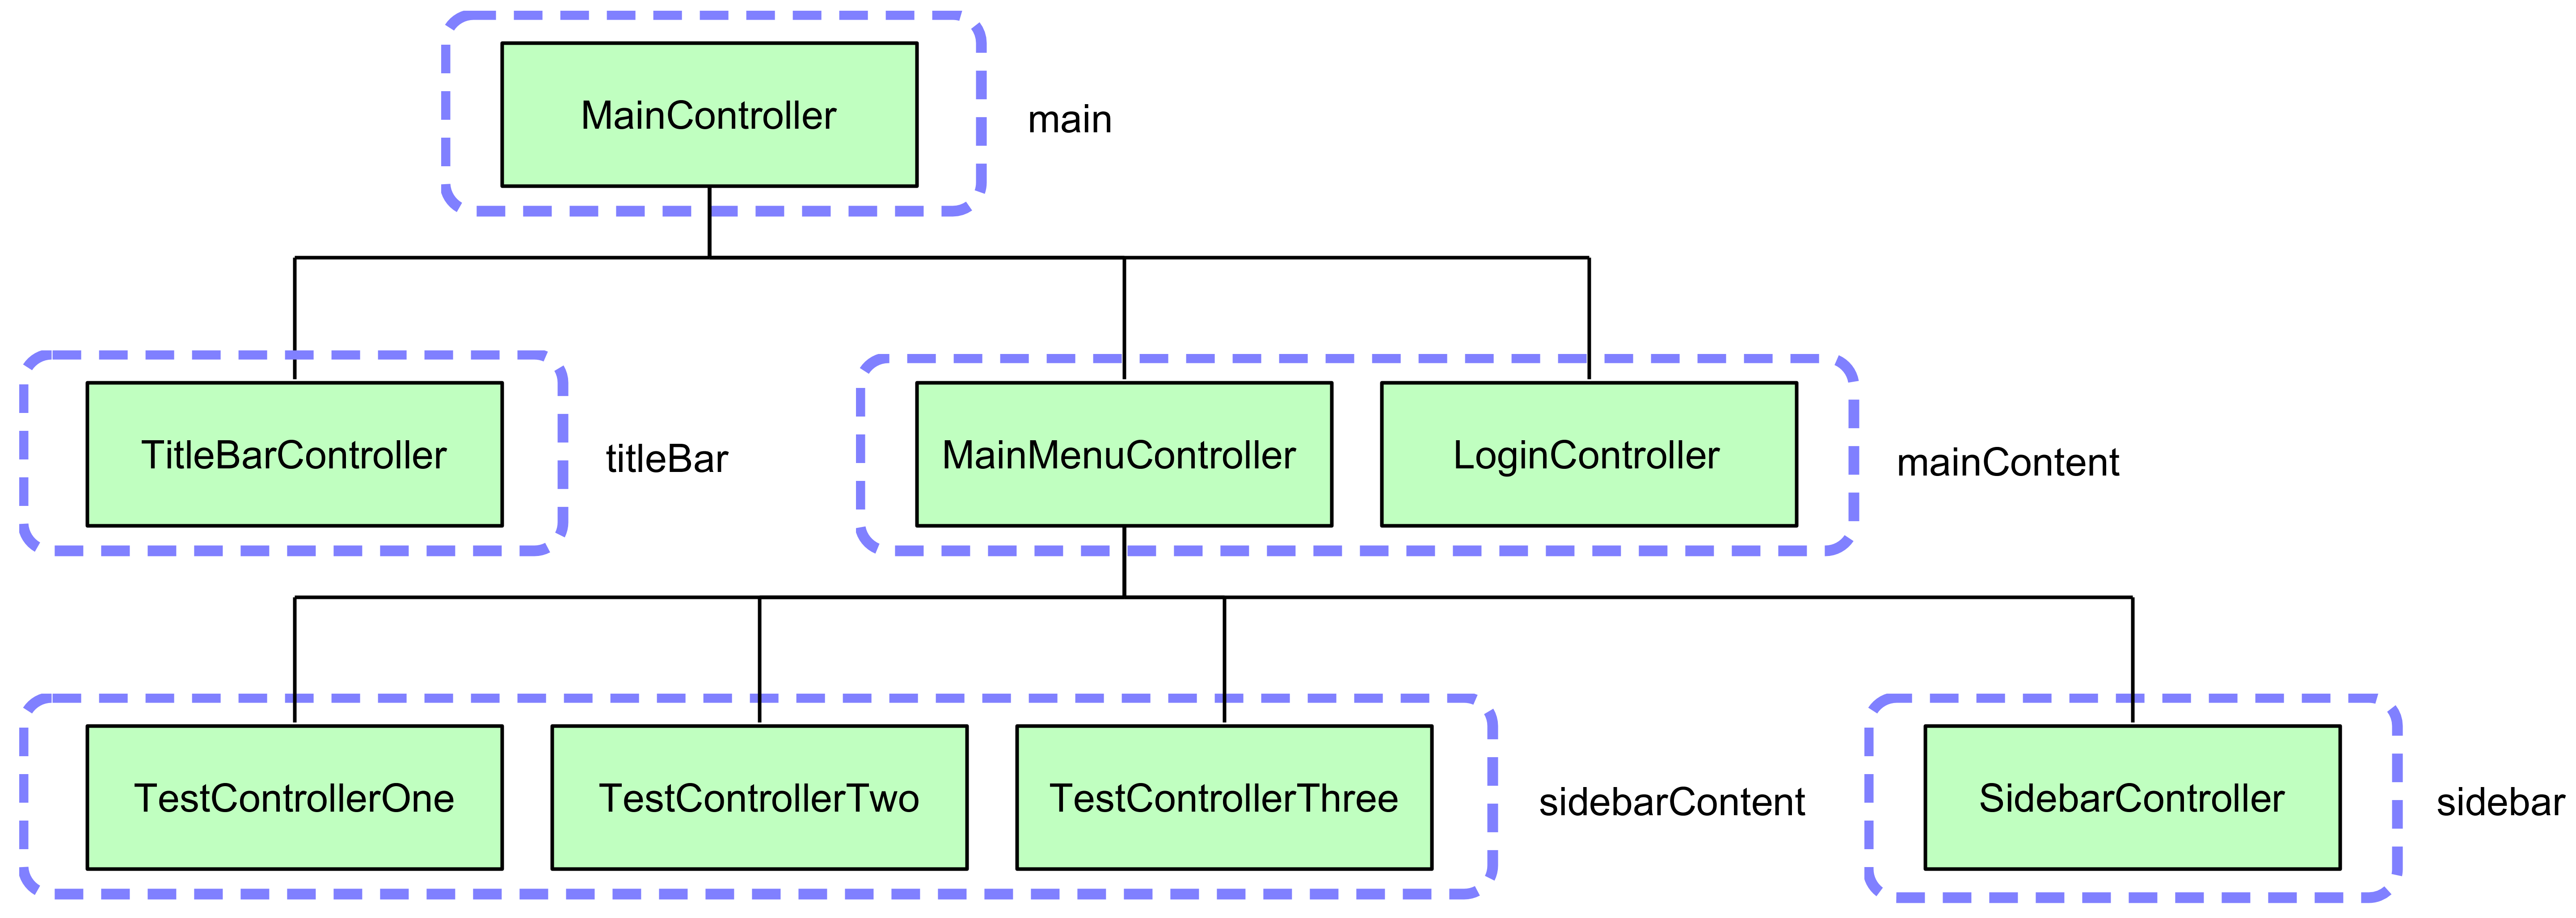
\includegraphics[width=\textwidth]{Abbildungen/Controller Relations.png}
	\caption{Diagramm -- Controller und Controllergruppen.}
	\label{fig:controller_relations}
\end{figure}
\subsection{Implementierung der Beispielanwendung}
Damit eine \texttt{SimpliFX} Anwendung als solche erkannt wird, muss eine Klasse definiert werden, welche als Einstiegspunkt dienen soll. Diese muss die Annotation \texttt{@ApplicationEntryPoint} aufweisen und als Parameter den Startcontroller (\texttt{MainController}) übergeben. Für die Abhängigkeitsinjektion mit Guice muss der Einstiegspunkt auch mit \texttt{@GuiceInjection} annotiert werden und die Klasse eines Guice-Moduls übergeben. Wie in der Einleitung bereits beschrieben, wird das Modul nur die Implementierung des Login Services bereitstellen (siehe \autoref{fig:login_service}). 
\begin{figure}[H]
	\centering
	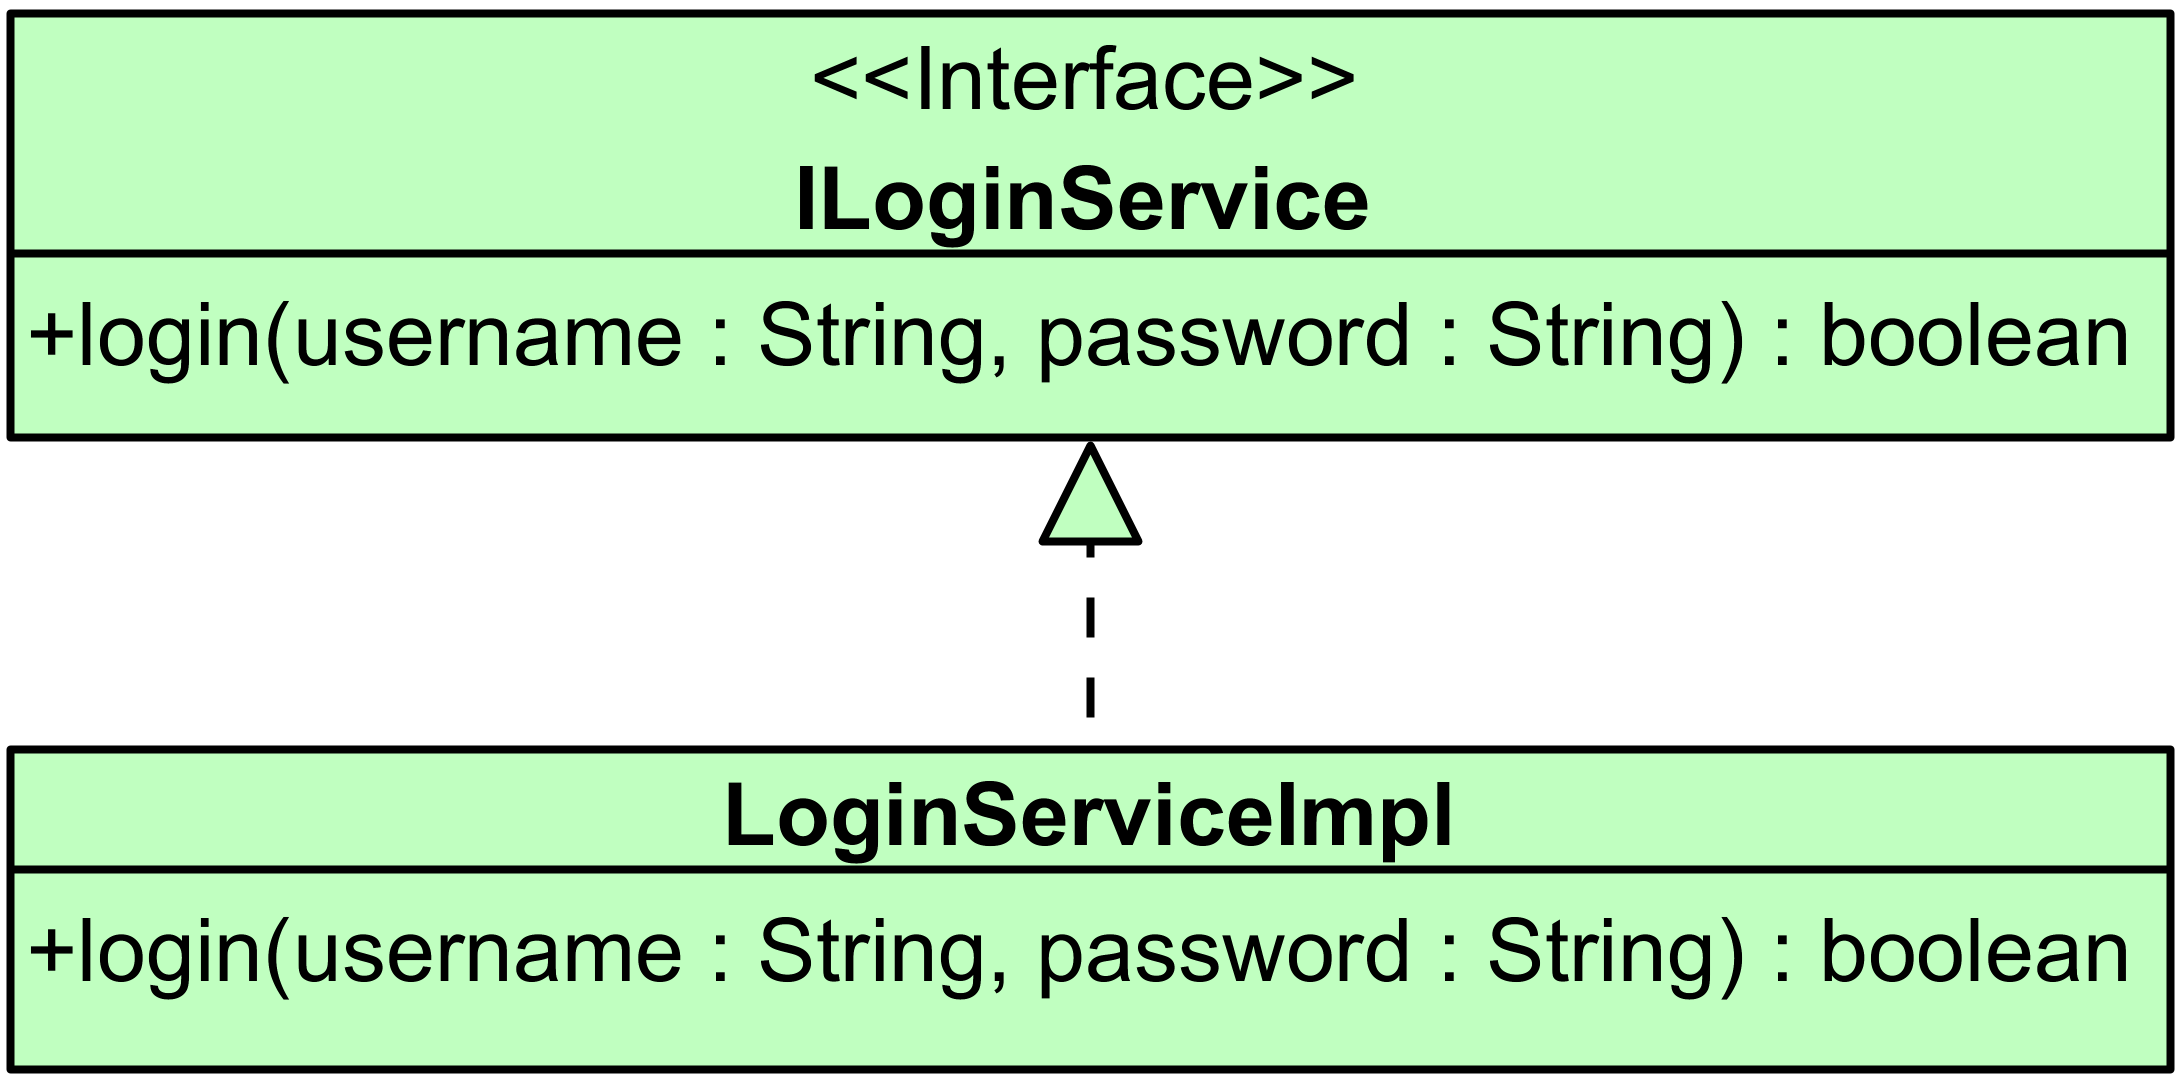
\includegraphics[width=\textwidth]{Abbildungen/Login Service.png}
	\caption{Diagramm -- Login Service.}
	\label{fig:login_service}
\end{figure}
\noindent Dazu werden noch Konfigurationsänderungen der \texttt{Stage} in Form von Symbol und Titeländerungen durchgeführt. Eine minimale Version des Einstiegspunktes ist in \autoref{lst:entry_point_demo} zu sehen. Dabei wird in Zeile Eins der Titel der \texttt{Stage} auf \texttt{Login} gesetzt und ein Symbol für die Fensterleiste angegeben. Danach wird der Hauptcontroller in der zweiten Zeile definiert, indem die jeweilige Controllerklasse als Parameter übergeben wird. Abschließend wird die Guice Kompatibilität aktiviert und ein Modul festgelegt (Zeile Drei).
\begin{figure}[H]
	\begin{lstlisting}[caption=Demo -- Minimaler Einstiegspunkt., captionpos=b, label=lst:entry_point_demo, numbers=left, xleftmargin=1.5em, framexleftmargin=1.5em]
#@StageConfig(title = "Login", icons = "icon.png")
#@ApplicationEntryPoint(MainController.class)
#@GuiceInjection(MainModule.class)
public final class DemoApplication {}
	\end{lstlisting}
\end{figure}
\noindent Für das Nutzen der dynamischen Übersetzung und der Konfigurationsschnittstelle müssen dem Einstiegspunkt zwei Felder hinzugefügt werden (\autoref{lst:fields_demo}). Außerdem sollen Subcontroller die Möglichkeit haben, den Titel der \texttt{Stage} abzuändern, weshalb die \texttt{titleProperty} als geteilte Ressource definiert wird und beim Start der Anwendung in einer \texttt{EventHandler} Methode gesetzt wird (\autoref{lst:event_method_demo}).
\begin{figure}[H]
	\begin{lstlisting}[caption=Demo -- Benötigte Felder., captionpos=b, label=lst:fields_demo]
#@ResourceBundle((@\tikzmark{resLeft}{}@)"lang.Messages"(@\tikzmark{resRight}{}@))
private II18N ii18N;

#@ConfigSource((@\tikzmark{conLeft}{}@)"config/connection"(@\tikzmark{conRight}{}@))
private Properties properties;

#@Shared
private SharedReference<StringProperty> (@\tikzmark{titleLeft}{}@)titleRef(@\tikzmark{titleRight}{}@);(@\begin{tikzpicture}[overlay,remember picture]
	\node[draw](resources) at (-0.5,3) {Pfad zum ResourceBundle};
	\node[draw](config) at (0.4,2) {Pfad zur Konfigurationsdatei};
	\node[draw](title) at (0.4,1) {Geteilte Ressource für Titel};
	\foreach \x/\y in {con/red,title/blue} {
		\DrawOverBar[-,\y,thick]{\x Left.north}{\x Right.north}
	}
	\DrawArrow[blue, in=280, out=-280]{title}{title}{0,-0.2}
	\DrawArrow[red, in=150, out=10]{con}{config}{-3.05,0.0}
	\renewcommand{\VerticalShiftForBar}{0em, -1.6ex}
	\renewcommand{\Stub}{0em, 0.3em}
	\DrawOverBar[-, green, thick]{resLeft.north}{resRight.north}
	\renewcommand{\VerticalShiftForArrows}{0, -1ex}
	\DrawArrow[green, in=215, out=-10]{res}{resources}{-2.3,-0.25}

\end{tikzpicture}@)
	\end{lstlisting}
\end{figure}
\begin{figure}[H]
	\begin{lstlisting}[caption=Demo -- Start EventHandler., captionpos=b, label=lst:event_method_demo]
#@EventHandler
private void onStart(StartEvent event) {
	// Titel Property setzen
    this.titleRef.set(event.getStage().titleProperty());
	// Stage zeigen
    event.getStage().show();
}
	\end{lstlisting}
\end{figure}
\noindent Zum Starten der Anwendung muss der Hauptcontroller korrekt deklariert werden und eine \texttt{main} Methode existieren, welche \texttt{SimpliFX\#launch} aufruft. Außerdem muss, aufgrund der Inkompatibilität zwischen JFoenix und Java 16, per Reflection-Schnittstelle eine \texttt{add-opens} Direktive vor der eigentlichen Initialisierung von \texttt{SimpliFX} und \texttt{JavaFX} hinzugefügt werden.\footnote{JFoenix Issue: \url{https://github.com/sshahine/JFoenix/issues/1052}} Der Einfachheit halber wird die \texttt{main} Methode in der \texttt{DemoApplication} Klasse deklariert (\autoref{lst:main_method_demo}).
\begin{figure}[H]
\begin{lstlisting}[caption=Demo -- \texttt{main} Methode., captionpos=b, label=lst:main_method_demo]
public static void main(String[] args) throws Exception {
    Reflection.addOpens("java.lang.reflect", "java.base",
			JFXTextFieldSkin.class.getModule());
    SimpliFX.launch();
}
	\end{lstlisting}
\end{figure}
\noindent Der funktionsfähige Einstiegspunkt der Anwendung ist noch einmal vollständig in \autoref{lst:entry_point_demo_full} dargestellt.\\
Wird zu diesem Zeitpunkt versucht, die Applikation zu starten, so wird diese mit einem Fehler terminieren, da der angegebene Hauptcontroller noch nicht erstellt und konfiguriert wurde.
\add{TODO CONTINUE}
\noindent...\\
...\\
...\\
\notebox{Die Höhe und die Breite einer Controllergruppe richtet sich immer nach dem aktuell angezeigten Controller. \texttt{SimpliFX} nutzt dazu das \texttt{prefHeight}- und \texttt{prefWidth} Attribut des jeweiligen Wurzelelementes. Ist kein solches Attribut gesetzt worden, werden Standardwerte genutzt.}
\section{Vergleich konventioneller Methoden mit entwickeltem System}
\label{vergleich_system_javafx}

\add{Vergleich konventioneller Methoden mit entwickeltem System}
